\chapter{Development environment design}\label{chap:editor}
This chapter describes the design of Dual's development environment.

\section{Overview}
The overall design tries to merge features of modern code editors, such as Brackets\cite{brackets_site}, Visual Studio Code\cite{vscode_site} or Atom\cite{atom_site} with visual programming language editors, such as the Blueprint Editor from Unreal Engine 4\cite{blueprint_editor}.

The environment is intended to work online, similarly to \acrlong{ide}s such as Codeanywhere\cite{codeanywhere_website} or Cloud9\cite{c9_website}. It should also work as offline, like Scratch's offline editor\cite{scratch_offline}.

\section{Design}

I set the following general goals that the designed development environment must meet:
\begin{itemize}
\item It should be easily usable with minimal effort from the user to install it or set it up.
\item The user interface and its idioms and metaphors\cite{ui_idioms} should be familiar to an experienced user and easy to learn for an inexperienced one.
\item The editor should support the text and visual representation and should provide an interface to add new representations.
\end{itemize}

\section{Design requirements}
In order to meet the above goals, I set down the following design requirements:
\begin{itemize}
\item The environment should be a web application.
\item The environment should have minimal external dependencies.
\item A folder is considered a project, similarly to modern code editors, such as Brackets or Visual Studio Code.
\item There should be a flexible global search faciltiy that can search through all editor options and menus.
\item The appearance of the visual representation should be customizable.
\end{itemize}

General layout considerations:
\begin{itemize}
\item The layout of the editor should conform to universaly accepted standards where possible.
\item There should be a menu bar at the very top of the screen.
\item The search facility should be available at all times. It should appear at the top of the screen.
\item There should be a console output area at the bottom of the screen.
\end{itemize}



The environment should have the following components:
\begin{itemize}
\item A project manager, which should be capable of managing local as well as remote projects.
\item A text editor with syntax highlighting, autocompletion, autoindentation, etc. for Dual. The text editor should conform to the design outlined in Section \ref{sec:est}.
\item A visual editor able to manipulate a visual representation of the EST  with autostructuring. It should also conform to the design outlined in Section \ref{sec:est}.
\end{itemize}

\section{Text editor}
The text editor should have 

\section{Visual editor}

\subsection{The visual representation}
The design of Dual's visual representation draws from many visual programming
languages. Analyzing these, we can observe several distinct approaches of which two particular designs are the most widespread and successful. These can be
described as ``line-connected block-based'' and ``snap-together block-based''
visual languages. The former family is exemplified by the Blueprints Visual
Scripting system of Unreal Engine 4\cite{blueprint} and the latter by MIT Scratch\cite{scratch, scratch_wikipedia}.

In order to address some of the most common criticisms of VPLs, outlined in Section \ref{sub:vpl_crit} I set the following general design requirements for the visual representation:
\begin{itemize}
\item It should combine the natural look of blocks connected with lines with the inherent structure of the Scratch-like languages.
\item It should be no harder to use than the text representation. Ideally a visual editor should add useful capabilities, without taking away these provided by text editors.
\end{itemize}

%TODO: criticisms of visual langs
% Existing visual languages are mostly criticized, because they fail to meet these basic criteria.

The visual representation should be mappable to the EST. There should be a distinguishable and manipulable visual element for every EST node. Such an element should contain a reference to the node (and vice versa).

There should be ways to perform the following actions with the visual editor:
\begin{itemize}
\item Insert new nodes into EST.
\item Remove existing nodes from the EST.
\item Modify existing nodes in the EST.
\item Replace existing nodes and subtrees in the EST.
\item Move nodes and subtrees to different locations in the EST.
\item Select and manipulate multiple arbitrary nodes and subtrees in the EST.
\end{itemize}

In short, the visual editor should provide ways to perform the same abstract operations on the EST that are possible when editing text and possibly more.

Some operations on raw text should also be reflected in the visual representation. For example the Find option. Searching through text should highlight the visual elements that correspond to the EST nodes that are connected to the text that contains the searched phrase. Regular expression based searching should also be possible. Replacing text with the Replace option should be reflected in the visual representation.

There should be a possibility to temporarily disable a representation by disconnecting it from the EST. Any changes made to other representations will then not be propagated to this representation. A disabled representation should become read-only until it is enabled. When it is enabled it should be updated to reflect the current state of the EST. At least one representation must be enabled at all times.

There should be a context-sensitive autocompletion feature. There should be an easily accessible library of functions and primitives with documentation.

User-defined functions should be added to this library upon definition and removed from it when they are removed from the source code.

\subsubsection{Structure}
The programmer could have the ability to alter the structure of the
representation, but he should not be required to constantly shape it. A
connected-block representations, such as the one in Unreal Engine 4 has no
mechanism that automatically structures the visual code similar to
autoindentation and other useful autostructuring features that evolved in code
editors over time and experience with using text-based programming
languages. This can be considered a regression on the visual editors' part.

The early designs show the following features that are not implemented in the
final prototype:
\begin{itemize}
	\item Names of the arguments are displayed instead of numbers if
          sensible.
	\item Names of types of variables
\end{itemize}

The colored squares with letters inside are actually placeholders for icons.  I
imagine a design, where the user is able to click on those icons and fold the
blocks into a more compact form, hiding the names and excessive text. This could
be done on the level of individual blocks, whole subtrees or the entire program
-- similar to code folding in text editors. This allows to have a big picture
and general relationships between nodes always visible and at the same time
gives an ability to focus on the details of the part at hand.

The text below the slots could be documentation comments associated with the
given argument. Their visibility could be toggleable through clicking on them,
on an individual or global basis, similarly to icons.

We can observe that there's a need to manipulate or set visual properties of
individual objects, clusters of objects/subtrees as well as the entire program
tree.


\begin{figure}[h!]
\centering 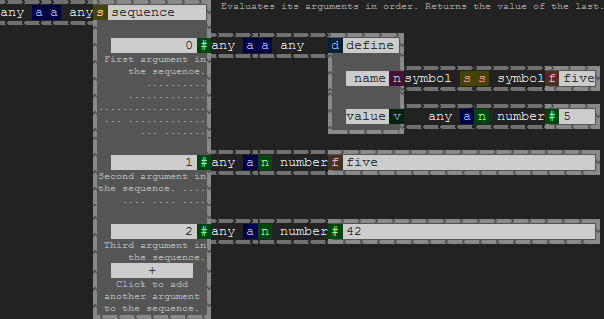
\includegraphics[width=0.9\textwidth]{design_3}
\caption{This design has the interesting property of visually illustrating the
  program flow with arrows.}
\label{fig:design_3}
\end{figure}


\begin{figure}[h!]
\centering 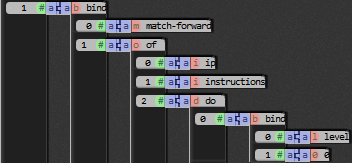
\includegraphics[width=0.9\textwidth]{design_4}
\caption{}
\label{fig:design_4}
\end{figure}



% UE4 editor



The templates could also be selected by the user from a visual library of puzzle
pieces, like the one in Scratch (Fig. \ref{fig:scratch}).
\begin{figure}[h!]
\centering 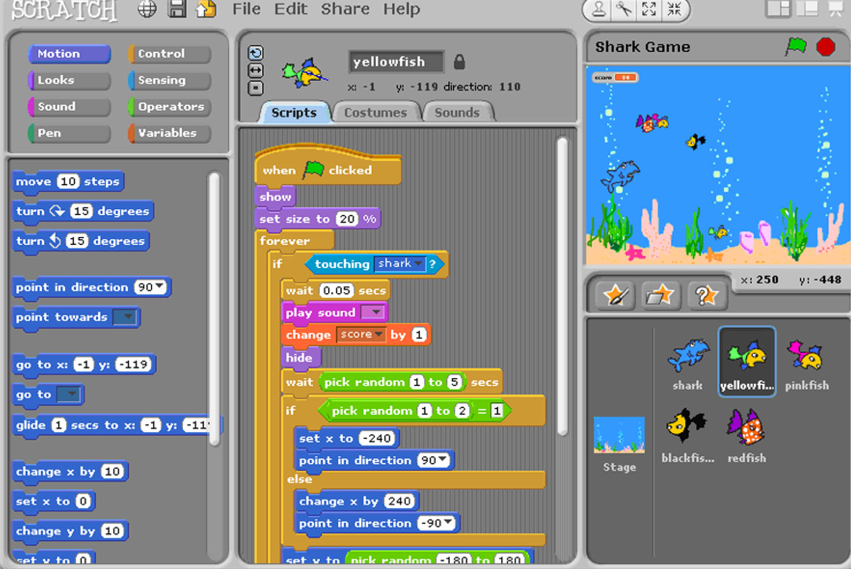
\includegraphics[width=0.9\textwidth]{scratch}
\caption{
    MIT Scratch programming language editor;
    screenshot from\protect\cite{fig_scratch}
}
\label{fig:scratch}
\end{figure}


\section{Visual editor}






\subsubsection{Flexibility}
The fact that the visual representation is composed purely out of HTML and CSS
Fully customisable with CSS

\subsubsection{Design}
\begin{figure}[h!]
\centering 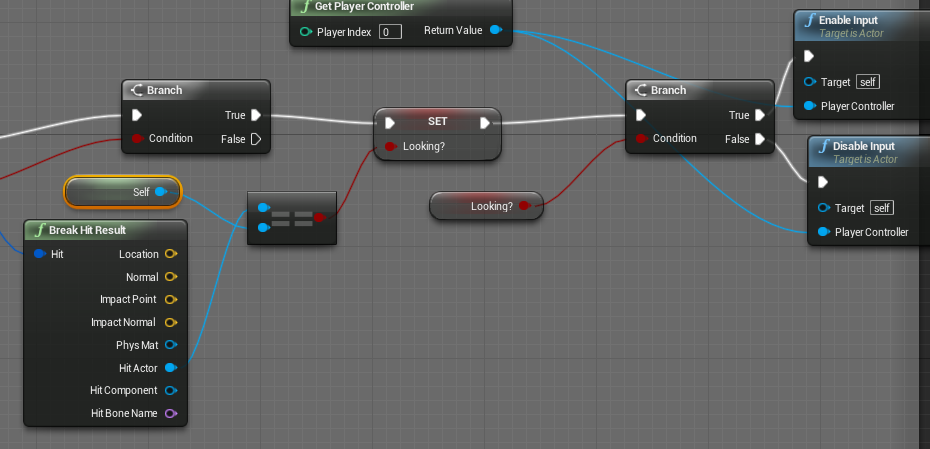
\includegraphics[width=0.9\textwidth]{blueprint_more}
\caption{}
\label{fig:blueprint_more}
\end{figure}

Many iterations:

\begin{figure}[h!]
\centering 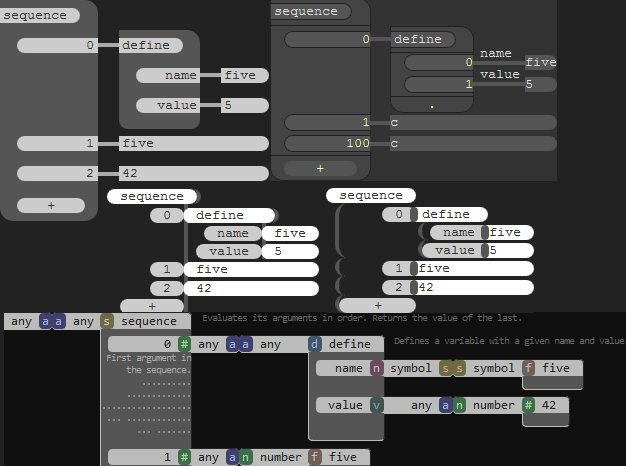
\includegraphics[width=0.9\textwidth]{designs_01234}
\caption{}
\label{fig:designs_01234}
\end{figure}

The visual form allows us to provide much more information about different
elements of the program. Spatially relate this information with these elements
through blocks and connections. Relate expressions with other expressions
through connections, which can also carry additional information.

We can distinguish the following visual elements:
\begin{itemize}
	\item Blocks, which represent expressions or individual nodes of the
          EST. Those in turn consist of:
	\begin{itemize}
		\item A header, which contains an icon and the name of the
                  expression's operator. Next to the header a documentation
                  comment might be displayed.
		\item Slots, which are the numbers or names of the arguments
                  followed by an icon; below these documentation comments could
                  be displayed.
		\item Possibly additional buttons, which could be used to add
                  more slots to variadic expressions.
	\end{itemize}
	\item Connections between slots and blocks, which could also contain
          some useful annotations. The proposed design places type annotations
          there. These consist of the name of the type followed by an icon that
          represents this type. Connections actually have two parts: one
          extending from a slot, which in this case would contain the argument's
          type annotation, and one extending from a block header, which would
          contain expression return value's type annotation.
\end{itemize}

Icons are a way to minimize the use of text to represent different entities

The text representation is very compact, which often is an advantage. This
advantage can be maintained by the visual representation by making all the
additional information optional. The user should have easy way of configuring
whether or not and what informations should be displayed. By folding some
textual elements into icons the visual representation could actually be made
more compact than the text form.

